
\title{Estimating the distance between people on public spaces based on neural networks}

\author{Laszlo Makara, Botond Varsanyi, Gergely Safran}

\maketitle

\tableofcontents
\listoffigures

\chapter*{Abstract}
As Covid-19 spread across the globe social distancing became more and more important and also the wearing of masks. Because with these restrictions we can successfully decrease the daily new cases, and minimaze the fullness of hospitals. If we could monitor the distance between people in shops and other public places, then we could let them know with speakers if they are too close to each other. The goal is a system that could be used in inner and outer places as well, and can also operate at night time and can measure the distances between people.
%A 2019-ben kirobbant Covid-19 járvány miatt kimndott fontosságot övez az egymástól tartott szociális távolság, valamint a maszk viselete. Hiszen ezek által lehet a fertőzöttségi számokat csökkenteni, ezzel a korházakra eső terhelést minimalizálni. Abban az esetben, ha tudnánk a kamera képeken monitorzálni a távolságot az egyes emberek között egy bolt esetén figyelmefelkeltéssel mint például a mikrofonba jelezhető a vásárolnak tartsák meg a kellő ajánlott távolságot. A cél egy olyan megoldás megalkotása ami kül és beltéren is tud üzemelni, valamint éjszaka is megtudja állapítani az egyes emberek között lévő távolságot.

\chapter{Introduction}
\label{intro}

Social distance calculating is though task on two dimensial images. There are a few possibilities in order to measure social distance. We tried to find a universal solution, meaning that it could esteem
distance in pictures and videos as well. We could achieve that with slicing the videos into frames and process the frames. After that
we teach our model with the frames. We chose the Detectron2~\cite{detectron2} model which can be used in Pytorch~\cite{pytorch} framework easily. Pythorch is a free access, open source framework developed by Facebook's AI team. We investigated other solutions how we could teach models in Tensorflow~\cite{tensorflow} for similar purposes, but because the simplicity of Pytorch we chose that. We also examined less intelligent options with OpenCV~\cite{opencv}, but this only uses outlines made by edge detection from Fourier transformation. There could be numerous problems about this which neural networks
can solve this is why we chose the path leading to neural networks.

%A sociális távolság meghatározásához több lehetősgünk van. Mi egy olyan megoldást kerestünk ami unverzális lehet olyan értelemben, hogy egyaránt tud képeken becslést és videón is végezni. Ezt úgy tudtuk elérni, hogy a vizsgált videó cikkelyt képszeletekre bontjuk és képként dolgozzuk fel az egyes képkockákat. Ezután a képkockákon végezzük el az általunk választott és tovább tanított modellel a feldolgozást. Az általunk választott model a Detectron2~\cite{detectron2} ami a Pytorh~\cite{pytorch} frameworkben könnyedén használható. A Pythorch framework a Facebook AI csapata által készített ingyenesen elérhető open-source keretrendszere. Megvizsgáltunk egyéb lehetőségeket is miként lehetne Tensorflow~\cite{tensorflow} alatt modelt betanítani hasonló megoldásokra, viszont a Pytorch egyszerűsége miatt erre esett a választásunk. Megvizsgáltuk az OpenCV~\cite{opencv}-vel való kevésbé intelligens megoldási lehetőségeket, ami pusztán csak a Fourier transzformációból adódó éldetektáció után előálló körvonalakból dolgozik csak. Ennél számos probléma felmerülhet, amit mind ki tud küszöbölni egy neurális hálózat, ezért is választottuk a neurális hálózat felé vezető utat. 

% \section{Flow Measurement Data}
\chapter{Implementation}
%A következő részben szeretnénk a megoldás implementálását bemutatni, ezek segítségével pontosabb rálátást biztosítani a megoldás működésére. 

In the next section we would like to introduce our implementation. This will provide a deeper insight of the solution.

\section{Detectron2}
Detectron2~\cite{detectron2} is Facebook AI Research's next generation software system that implements state-of-the-art object detection algorithms. It is a ground-up rewrite of the previous version, Detectron, and it originates from maskrcnn-benchmark. The training of the system will be done with pictures and tags and masks for the pictures from a database. These tags provide accurate rectangle containers for objects, and the masks define the arcs of shapes. In the \ref{fig:det2} figure we can see that the objects have containers and are masked.
%A rendszer tanítása képekből és ahhoz tartozó maszk illetve tageleő adatbázisból el, ezek a tagek pontos téglalap körülhatárolást adnak az egyes objektumokról, valamint a maszkok specifikáljak az alakzatok pontos ívét. A \ref{fig:det2} ábrán jól látható ahogy az egyes objektumok pontosan körül vannak határolva és maszkolva vannak. 


\begin{figure}[!ht]
\centering
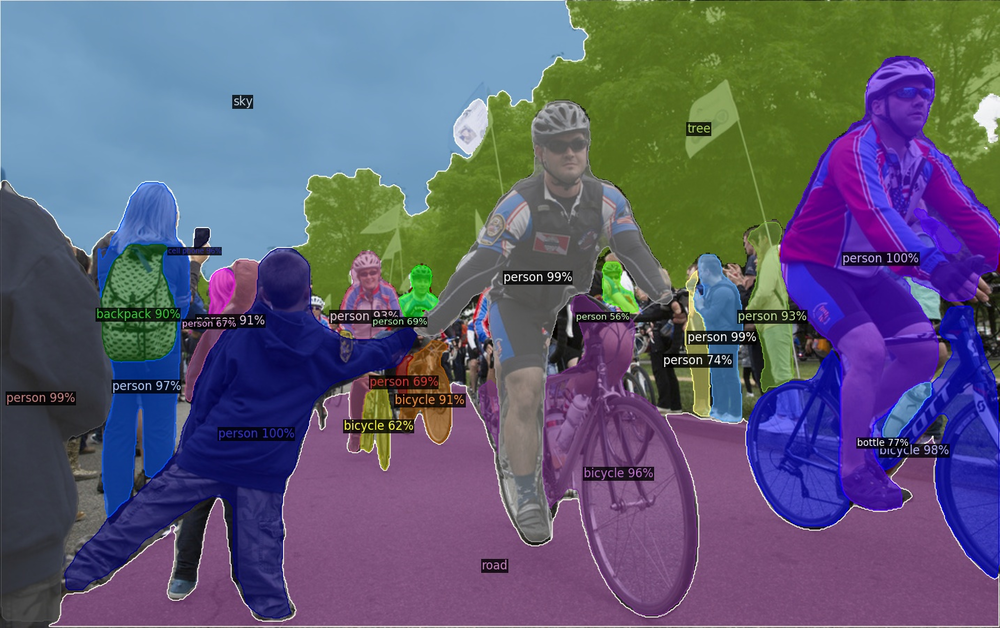
\includegraphics[width=85mm,keepaspectratio]{fig/66535560-d3422200-eace-11e9-9123-5535d469db19.png}
\caption{Detecting objects on image\cite{detectron2}}
\label{fig:det2} 
\end{figure}

\section{Datasets}
For teaching the model further, we used the free Kaggle~\cite{kaggle} databases. The databeses available here are pre-tagged in the format that we need. But this alone is not sufficient, from this our model can’t feed, so we have to convert this to the appropriate format and we have to generate the describing Json files. We used the free online software Roboflow for this. Roboflow~\cite{roboflow} is capable of generating the datasets from the input data. In case of teaching Detectron2 we need Coco type data. So we generated the Coco dataformat from the pictures gathered on Kaggle.
%A model további tanításához az ingyenesen elérhető Kaggle~\cite{kaggle} adatbázisokat használtuk. Az itt elérhető adatbázisok már előre fel vannak tagelve az általunk szükséges formátumban. Viszont ez önállóan még nem lenne elég, ebből a választott modellünk nem tudna táplálkozni, ezért át kell alakítani megfelelő formátumuvá és le kell generálni a hozzá tartozó Json leíró fájlokat. Ezt az ingyenesen használható online Roboflowwal~\cite{roboflow} végeztük. A Roboflow képes a beadott adatok alapján a szükséges formátumban kigenerálni az adathalmazt. A Detectron2 esetében a tanításhoz Coco típusú adatok szükségesek. Ezért ezzel az eszközzel kigeneráltuk Coco adatformátumba a Kaggle oldaláról begyűjtött képeket. A \ref{fig:roboflow} ábrán jól látható milyen típusú adatok és körülhatárolások tartoznak az egyes képekhez.

\begin{figure}[!ht]
\centering
\includegraphics[width=35mm,keepaspectratio]{fig/roboflow_image.png}
\caption{Roboflow tagged images}
\label{fig:roboflow} 
\end{figure}

\section{Distance projection}
For measuring the correct distance on the image of the camera, the 3 dimension space must be reconstructed from the 2 dimension image.  In order to do this we need to know the focal length and the viewing angle of the camera, which is referred to as "POV”. The letter of focal length is "f” here. In case coordinates X and Y could be determined precisely, we could calculate the distance between the two pedestrian using the Eucledian distance calculus. The scaling is described by these functions:
%A pontos távolság meghatározásához a kamera képen vissza kell állítani a két dimenziós képből a három dimenziós teret. Ahhoz, hogy ezt meg tudjuk tenni ismernünk kell a kamera fokális távolságát, valamint a kamera által bezárt látószöget amire POV-ként szoktak referálni. A kamera fokális távolságát az $f$ jelöli. Abban az esetben ha sikerült megfelelőn az X,Y koordináták meghatározása a három dimenziós térben már kitudjuk hagyományos Euklédeszi távolság mérésvel számolni a két gyalogos által tartott szociális távolságot. Az átskálázás az alábbi függvényekkel írhatóak le.

\begin{equation}
    X = u*\frac{Z}{f}
\end{equation}

\begin{equation}
    Y = v*\frac{Z}{f}
\end{equation}
The social distance between the two person in 3 dimension space is calculated below
%A két fő között megjelenő szociális távolságot az alábbiak szerint tudjuk kiszámolni a három dimenziós térben.

\begin{equation}
    \Delta d=\sqrt{(X_{1}-X_{2})^2 + (Y_{1}-Y_{2})^2+(Z_{1}-Z_{2})^2}
\end{equation}

Unfortunately we could not implement this, because the specifications of the publicly and freely accessible cameras are not available.
Because of that we could only estimate the focal distance and the angle of view. Instead of that we used realtive distance determination.
The distance between two pedestrians can be determined with two given threshold values. Ad hoc testing lead us to a relatively good solution.
The problem with this is that the algorithm won't work properly with pedestrians in the distance. If we would like to release this for
industrial purposes, the implementation of that is necessary beside of knowing the exact specifications of the camera we use.
%Sajnos a végleges megoldásban ezt nem tudtuk implementálni, mert a nyilvánosan és ingyenesen felhasználható kamera képekhez tartozó specifikációk nem ismertek. Ezáltal a fokális távolságra, valamint a betekintési szögre csak becslést tudnánk adni. Ehelyett a végleges megvalósításban relatív távolság meghatározással dolgoztunk. Két küszöbértéket megadva lehet megállapítani a két ember közötti szociáis távolságot, ennek egy viszonylagosan jó meghatározásához ad-hoc tesztelés vezetett el. Probléma ebben az esetben, hogy a távolban lévő személyek esetén, viszont nem fog megfelelően működni így az algoritmus. Az iparban való alkalmazhatóságához, mindenképpen meg kell valósítani ezt a funkciót amellett, hogy teljes ismeretébe legyünk a kamerához tartozó specifikációkról.

\section{Image slicing}
%A videót képekre való bontása az OpenCV~\cite{opencv} nyílt forráskodó Python könyvtár segítségével valósítottuk meg. A bementi videónak megvizsgáljuk a képfrissítési rátáját és eszerint mintavételezzük a képeket. Itt fontos megemlíteni, hogy abban az esetben ha magas a képfrissítés akkor az egyes elmozdulási vektorok az embereknek kicsi, ezáltal az erőforrás feleslegesen van terhelve, csökkenteni kell a mintavétel méretét. Érdemes lenne megvizsgálni, hogyan lehet dinamikusan korrigálni a mintavételi rátát az elmozdulások függvényében, abban az esetben amikor az elmozdulási vektorok kicsik csökkentjük a mintavételi frekvenciát, amikor pedig nagy növeljük egy előre deffiniált küszöbértékig a mintavételi frekvenciát ami nem haladhatja meg a videó képfrissitését. A videó képfrissítését meghaladó frekvencia esetén redundáns képmetszeteket állítannánk elő amelyek plussz információt nem hordoznának magukban. 
The slicing of the videos into frames was done with the open-source Python library, OpenCV~\cite{opencv}. We check the framerate of the input video and we take picture samples according to that. It is important to mention here, that if the framerate is high then the movement vectors are small of the people and the resources are burden unnecessarily, and decreases the number of samples. It would be worth to investigate, how could we correct the sample rate depending on the movement. If the movement vectors are small we decrease the sampling frequency, and if it is high we increase the sampling frequency until we hit a threshold but it can not exceed the video's framerate. If we would exceed the framerate of the video we would produce redundant image sections carrying no additional information.

\begin{figure}[!ht]
\centering
\includegraphics[width=85mm,keepaspectratio]{fig/h246_composite.png}
\caption{Generating image flows from video}
\label{fig:image_slicing} 
\end{figure}

\chapter{Research}
There are quite a few other solutions published in 2020 regarding how social distancing could mitigate the risk of getting infected.
We used some of the ideas to figure out where we want to go. The \cite{deepsocial} is trying to use a whole different aspect to
determine the distance between two people: they try to transform the picture of what the camera sees, into a view that a bird would
see, like the system would watch the pedestrians from above. With this projection to know the depth of the image is not needed, but
we lose informations such as the height of the person. Also this does not carry important information because we only interested in
the distance between two pedestrians. The results using the YOLOv3 and DeepSOCIAL model were not significantly different. The \cite{visbased}
also uses a projection like the previous. But in this case they focus on the relationship between the pedestrians and the probability
of getting infected and not on the actual distances between two people. The \cite{socdist} relying on YOLOv3 also builds the solutions
seen in \cite{deepsocial}, talking about the bird view aspect. This solution does not include estimating the probability of infection
and does not handle families or groups neither. The \cite{vissoc} is a must know about this topic. Basically it defines the public spheres
of people and the probability of infection connected to that. The sphere becomes distorted depending on the movement vector of the pedestrian, 
like a Doppler effect that should be taken into account. \cite{8717277} also offers an exceptional solution. They use polinomial approximitaion
to determine the distance between two people, but this does not solve the problem of groups alone. Investigating and recognizing groups and
families introduce a new problem in this topic. But this should be solved if the product want to be useful in real life. It should be handled for
example if a child in a family is cycling around the family, and the distance between them changing dynamically. Because in this case the system should
not go off.
%Számos hasonló megoldást publikáltak a 2020-as év folyamán amikben a kockázat csökkentésének lehetőségét vizsgálják a szociális távolság megállapításában. Sok ikhletet a pontos irány tekintetében ezekből meritettünk. A \cite{deepsocial} egy teljesen más megközelítésből figyeli meg a problémát az emberek közötti távolság megállapítására, megpróbáljak a kamera képet leképezni egy madártávlatbeli képpé, mintha felülről szemléné a rendszer a gyalogosokat. Ezzel a projekcióval élve nem szükséges a kép mélységét ismerni, igaz igy olyan információkat vesztünk el mint a gyalogos magassága, viszont ez esetünkben nem számít csak a két gyalogos közötti távolság relatíve pontos meghatározása érdekel minket. A megoldás YOLOv3 és DeepSOCIAL modelt felhasználva is kirtékeltél szignifikáns különbség teljesítmény terén nem nagyon van a kettő model között.
%A \cite{visbased} esetében egy hasonló felsőnézeti leképzést készítenek, ahol inkább jobban összpontosítanak az egyes emberek közötti kapcsolatok megvizsgálásával és a fertőzés kockázati valószínűségével mint a tényleges táv rekontstrukciójával. 
%YOLOv3-ra építő megoldás \cite{socdist} ami a \cite{deepsocial}-ban látott megoldásokra épít a madárlesi távolság rekonstrukciójában. Ez a megoldás nem foglal magában becslést a fertőzés valószínűségére és továbbá nem kezeli az egybe tartozó családok/csoportok kérdéskörét sem. 
%A \cite{vissoc} egy alap műként tekinthető ebben a témakörben, gyakorlatilag deffiniálja egy gyalogos publikus szféráját, illetve az ahhoz tartozó fertőzési kockázatokat. A gyalogos szférája az adott sebesség vektor függvényében eltorzul, mint egy Doppler effektus amivel szálmolni kell. 
%Hasonlóan egy kiváló megoldást kinál a \cite{8717277} amiben polinomiális közelítés segítségével állapitják meg két gyalogos közötti távolságot, viszont ez sem kinál önmagában megoldást a csoportok megállapítására. 
%A csoportokkal és családokkal kapcsolatos megállapitások új kutatási teret vet fel ebben a problémakörben. Ahhoz, hogy ez egy iparban használható alkalmazás legyen mindenképp vizsgálni kell a családok és csoportok szituációját. Le kell tudni kezelni azt az esetet amikor egy családban található kisgyermek elbiciklizik egy pár méterre a családtól majd vissza úgy, hogy ne jelezzünk veszélyt ekkor a gyermek és családról-

\chapter{Solution}
%Az elkészült megoldásról egy képkocka a \ref{fig:distance} ábrán látható. A képen három különböző szín látható. A kék azt jelzi, hogy az adott gyalogos biztonságban van nincs a közelében a küszöbértéken belüli másik gyalogos. A sárga szín azonosítja a veszélyesség lehetőségét, ez még maszk esetén nem feltétlen elégséges a fertőzés átadásához, viszont meg van már a kockázata. Ekkor sárga vonallal vannak összekötve az adott felek, jelezve a veszély forrássait. A piros színnel jelölt a más veszélyes zonában elhelyezkedő gyalogosokat, itt már előfordulhat az az eset is amikor egy maszk viselése amely nem rendelkezik elég réteggel nem állítja meg a fertőzés tovább terjedését. Fontos megint megjegyezni, hogy a térbeli elhelyezkedések esetén előfordulhat hibás becslés, mivel nem ismertük a kamerával kapcsolatos pontos specifikációkat. 

We can see a frame of the final solution in the \ref{fig:distance} figure. In the picture we can see three different colours. Blue indicates that the given pedestrian is in safe: there is nobody around them nearer than the given threshold. Yellow indicates a warning: in case of proper mask wearing the pedestrian is not in danger but there is the possibility of getting infected. In this case the pedestrians are connected with a yellow line indicating the possibility of danger. Red indicates pedestrians in danger zone. In these cases maybe proper mask wearing is not enough to avoid getting infected. It is important to mention, that there could be a wrong estimation of distances because of the 3 dimensional aspects due we do not know the exact specifications of the camera.

\begin{figure}[!ht]
\centering
\includegraphics[width=85mm,keepaspectratio]{fig/distance_on_image.png}
\caption{Estameted distances}
\label{fig:distance} 
\end{figure}

\section{Train}
The output of the teaching is shown on figure \ref{fig:train}. The database gathered from Kaggle consisted of people and statues. The statues were tagged “person like” and real people were tagged as “person”. In the teaching set there were 281 people and 288 statues. The teaching took about one and a half hour on the Google Colab platform, where an NVIDIA Tesla K80 video card was used. We used the Google Colab platform because in our personal experience it’s the best for running Python Notebook and the system gives us a much stronger dedicated graphics card than the ones in our personal computers. The consumer graphics cards are not made for this.

%A \ref{fig:train} ábrán látható a tanítás kimenete. A Kaggle-ről begyüjtött adatbázis embereket valamint szobrokat tartalmazott. A szobrok person-like míg a valós emberek person-ként lettek feltagelve. A tanító mintában 281 darab ember és 288 szobor található. A tanítás maga körbelül egy- másfél órát vett igénybe a Google Colab felületén, ahol NVIDIA Tesla K80 kártyával történt a tanítás. Azért a Google Colab felületét választottuk, mert személyes tapasztalatunk ez a legjobb Python Notebook futtatásához, valamint sokkal erősebb dedikált grafikus vezérlőt bocsájt rendelkezésünkre a rendszer, mint amivel a személyi számítógépünk rendelkezik. A hagyományos otthoni felhasználásra szolgáltatott grafikus vezérlők nem megfelelőek erre a célre. 

\begin{figure}[!ht]
\centering
\includegraphics[width=85mm,keepaspectratio]{fig/train.png}
\caption{Train results}
\label{fig:train} 
\end{figure}

\section{Validation}
The validation dataset is also from Kaggle. We used the 70 percent of the collected data for training, 20 percent to validating, and kept 10 percent for testing. In the test datas we can see that the model recognize  with a 66\% accuracy in the person category while the person-like category was with a 71\% accuracy. If we could train the model more and with more data, we could achive an even better result, recognizing pedestrians more accurately. Unfortunately due to lack of time and the limits of Google Colab (storage and memory) we could not achive that. In order to develop we should use more powerful resources such as that Azure offers in their Machine Learning Studio service.
%A validációs adatbázis ugyan csak a Kaggle-ről származik. A beszerzett adatok 70\%-át használtuk fel tanító adatnak 20\%-át validációs adatnak és 10\%-át tartottuk meg teszt adatnak. A teszt adatokon jól látszik, hogy a person categóriába 66\%-os bizonyosságal döntött megfelelően a rendszer míg a person-like esetében ez az érték 71\%-os. Abban az esetben ha ezt tovább tanítanánk még több adattal még jobb eredményt tudnánk elérni, ezzel is pontosabban ráismerve a gyalogosokra. Sajnos az idő rövidsége miatt és a Google Colab által nyújtott korlátos szolgáltatások (tárhely és memória) miatt ez nem állt rendelkezésünkre. Ahhoz, hogy ezt tovább tudjuk fejleszteni szükségeszerűen használnunk kellene erősebb erőforrásokat, olyanokat mint amit az Azure kínál a Machine Learning Studio szolgáltatásaiban. 


\begin{figure}[!ht]
\centering
\includegraphics[width=85mm,keepaspectratio]{fig/validation.png}
\caption{Validation results}
\label{fig:validation} 
\end{figure}

\subsubsection{Google Colab}
Colaboratory, or "Colab"~\cite{colab} for short, allows users to write and execute Python in their browser, with zero configuration required, free access to GPUs and easy sharing.

\subsubsection{Azure Machine Learning Studio}
Azure Machine Learning is a separate and modernized service that delivers a complete data science platform. It supports both code-first and low-code experiences. Azure Machine Learning studio~\cite{studio} is a web portal in Azure Machine Learning that contains low-code and no-code options for project authoring and asset management.


\chapter{Conclusion}
%Az eszköz még további fejlesztésekre szorul. A felhasznált videóval kapcsolatban nem álltak elő olyan információk mint a kamera látószöge, vagy fokális távolsága. Ezek miatt sajnos a három dimenzióból a két dimenzióba való projekciót nem tudjuk megtenni. Ez azért lenne szükséges mert igy megbecsülhető lenne a képen látható mélységek és ezáltal pontosan meg lehetne állapítani az Euklédeszi távolságot, amit korábban a leírásokban bemutattunk. Ahhoz, hogy ezt az alkalmazást ipari környezetben lehessen alkalmazni mindenképp meg kell vizsgálni ennek a megvalósítási lehetőségeit. Érdemes lenne továbbá más nem a Detectron2-re építő model-t megvizsgálni és összevetni az egyes esetekben a teljesítményét az alkalmazásnak. Tovább fejlesztési lehetőségként meglehetne vizsgálni a szobrok esetén való feltanítását a modelnek. A jelenelegi megoldás esetén például látható, hogy a képernyő bal szélén egy szobor található, amit sokszor emberként ismer fel a rendszer. Abban az esetben, ha jól feltudnánk tanítani a szobrok vizsgálatára akkor ezeket a szituációkat kiszűrnénk és jobban lehetne a közterületeken alkalamzni. Valamint a korábban bemutatott megoldási tervezetben említettük a családtagok felismerését, hiszen ebben az esetben nem kell jelezzen a rendszer, nem szükséges számukra a kellő szociális távolság tartása, viszont ez nem került megvalósításra, adandóan a pontos távolság meghatározásának lehetőségéből és a pontatlan felismerésből.
The tool needs some future developments and enhancements. There was no information such as the angle of view of the camera, or the focal distance for the footage that we used. Because the lack of these informations we could achieve the projection from 3 dimension to 2 dimension. This projection would be necessary to esteem the depths of the pictures and with that the eucledian distance could be calculated accurately, that we introduced before in our description. If we would like to apply the solution in the real world we have to solve the problems mentioned before.  Furthermore, it would be worth to investigate other models and not only that relies on the Detectron2 and compare the performances of those. A development
possibility is to teach the model about statues: for example in our current solution we can see a statue in the left of the screen, which sometimes is recognized as a human. If we could teach the model about statues then it would be more reliable on public squares. We mentioned before that we plan to recognize families, because the system should not
go of because of a family since they are not required to keep distance from each other. But this feature was not implemented due to innacurete recognition.